%%%%%%%%%%%%%%%%%%%%%%%%%%%%%%%%%%%%%%%%%%%%%%%%%%%%%%%%%%%%%%%%%%%%%%%%%%%%%%%%
%2345678901234567890123456789012345678901234567890123456789012345678901234567890
%        1         2         3         4         5         6         7         8

\documentclass[letterpaper, 10 pt, conference]{ieeetran}  % Comment this line out
                                                          % if you need a4paper
%\documentclass[a4paper, 10pt, conference]{ieeeconf}      % Use this line for a4
                                                          % paper

%\IEEEoverridecommandlockouts                              % This command is only
                                                          % needed if you want to
                                                          % use the \thanks command
%\overrideIEEEmargins
% See the \addtolength command later in the file to balance the column lengths
% on the last page of the document



% The following packages can be found on http:\\www.ctan.org
\usepackage{graphics} % for pdf, bitmapped graphics files
\usepackage{graphicx}
\usepackage{subcaption}
\usepackage[utf8]{inputenc}
\usepackage{acronym}
\usepackage{color}

%\usepackage{epsfig} % for postscript graphics files
%\usepackage{mathptmx} % assumes new font selection scheme installed
%\usepackage{times} % assumes new font selection scheme installed
\usepackage{amsmath} % assumes amsmath package installed
\usepackage{amssymb}  % assumes amsmath package installed
\usepackage{amsthm} % need to define new theorem styles
\usepackage{mathrsfs} % Fancy font
\usepackage{mathtools}
\usepackage{tikz}
\usetikzlibrary{shapes.geometric, arrows, angles, quotes}

\theoremstyle{definition}
\newtheorem{definition}{Definition}
\newtheorem{example}{Example}
\newtheorem{fact}{Fact}
\newtheorem{corollary}{Corollary}
\theoremstyle{theorem}
\newtheorem{theorem}{Theorem}
\DeclarePairedDelimiter\ceil{\lceil}{\rceil}
\DeclarePairedDelimiter\floor{\lfloor}{\rfloor}

\title{%\LARGE \bf
Improving Physical-Layer Security through Random Beamforming
}

%\author{ \parbox{3 in}{\centering Huibert Kwakernaak*
%         \thanks{*Use the $\backslash$thanks command to put information here}\\
%         Faculty of Electrical Engineering, Mathematics and Computer Science\\
%         University of Twente\\
%         7500 AE Enschede, The Netherlands\\
%         {\tt\small h.kwakernaak@autsubmit.com}}
%         \hspace*{ 0.5 in}
%         \parbox{3 in}{ \centering Pradeep Misra**
%         \thanks{**The footnote marks may be inserted manually}\\
%        Department of Electrical Engineering \\
%         Wright State University\\
%         Dayton, OH 45435, USA\\
%         {\tt\small pmisra@cs.wright.edu}}
%}

%\author{Telmo Fernandes$^{1}$, Jack Pfister$^{2}$, Marco Gomes$^{1}$, João P. Vilela$^{3}$ and Willie K. Harrison$^{2}$% <-this % stops a space
%\thanks{*This work was not supported by any organization}% <-this % stops a space
%\thanks{$^{1}$Instituto de Telecomunicações, Department of Electrical and Computer Engineering
%        University of Coimbra, Coimbra, Portugal
%        }%
%\thanks{$^{2}$Department of Electrical and Computer Engineering,
%        University of Colorado Colorado Springs, Colorado Springs, CO, 80923
%        }%
%\thanks{$^{3}$CISUC and Department of Informatics Engineering,
%        University of Coimbra, Coimbra, Portugal
%        }%
%}

\author{\IEEEauthorblockN{Darren Lund\IEEEauthorrefmark{3},
		Marco A. C. Gomes\IEEEauthorrefmark{1},
		Jo\~{a}o P. Vilela\IEEEauthorrefmark{2}, and
		Willie K. Harrison\IEEEauthorrefmark{3} \\
	}
	\IEEEauthorblockA{\IEEEauthorrefmark{1}Instituto de Telecomunica\c{c}\~{o}es, Department of Electrical and Computer Engineering, University of Coimbra, Portugal}
	\IEEEauthorblockA{\IEEEauthorrefmark{2}CISUC and Department of Informatics Engineering, University of Coimbra, Portugal}
	\IEEEauthorblockA{\IEEEauthorrefmark{3}Department of Electrical and Computer Engineering, Brigham Young University, UT, USA\\ Emails: darrenlund@byu.edu, marco@co.it.pt, jpvilela@dei.uc.pt, willie.harrison@byu.edu }
}

\acrodef{ARQ}[ARQ]{Automatic Repeat reQuest}
\acrodef{BEC}[BEC]{Binary Erasure Channel}
\acrodef{BER}[BER]{Bit-Error Rate}
\acrodef{SINR}[SINR]{Signal-to-Interference and Noise Ratio}
\acrodef{DMC}[DMC]{Discrete Memoryless Channel}
\acrodef{AWGN}[AWGN]{Additive White Gaussian Noise}
\acrodef{BSC}[BSC]{Binary Symmetric Channel}
\acrodef{BEWC}[BEWC]{Binary Erasure Wiretap Channel}
\acrodef{ICSHK}[ICSHK]{Interleaved Coding for Secrecy with a Hidden Key}
\acrodef{MAP}[MAP]{Maximum A Posteriori}
\acrodef{ML}[ML]{Maximum Likelihood}
\acrodef{LDPC}[LDPC]{Low-Density Parity-Check}
\acrodef{QPSK}[QPSK]{Quadrature Phase-Shift Keying}
\acrodef{KL}[KL]{Kullback-Leibler}
\acrodef{PEC}[PEC]{Packet Erasure Channel}
\acrodef{PEWC}[PEWC]{Packet Erasure Wiretap Channel}
\acrodef{PEP}[PEP]{Packet Erasure Probability}
\acrodef{AMPEP}[AMPEP]{Average Minimum Packet Erasure Percentage}
\acrodef{OSI}[OSI]{Open Systems Interconnection}
\acresetall

\graphicspath{{./../}}

\tikzstyle{communicator} = [rectangle, rounded corners, minimum width=1.5cm, minimum height=1cm, text centered, draw=black, fill=blue!30]
\tikzstyle{proc} = [rectangle, rounded corners, minimum width=1cm, minimum height=1cm, text centered, draw=black, fill=red!30]
\tikzstyle{chan} = [rectangle, rounded corners, minimum width=2cm, minimum height=1cm, text centered, draw=black, fill=green!30]
\tikzstyle{arrow} = [thick,->,>=stealth]
\tikzstyle{antenna} = [circle, radius=0.25cm, text centered, draw=black, fill=gray!30]
\tikzstyle{connect} = [thick,-,>=stealth]

\begin{document}



\maketitle
%\thispagestyle{empty}
%\pagestyle{empty}


\renewcommand{\thefootnote}{}
\footnotetext{This work was partially funded by the following entities and projects: the
	US National Science Foundation (Grant Award Number 1761280), the FLAD 
	project INCISE
	(Interference and Coding for Secrecy), project
	SWING2 (PTDC/EEI-TEL/3684/2014), funded by Fundos Europeus Estruturais 
	e de Investimento (FEEI) through Programa Operacional Competitividade 
	e Internacionaliza\c{c}\~{a}o -  COMPETE 2020 and by National Funds from FCT - 
	Funda\c{c}\~{a}o para a Ci\^{e}ncia e a Tecnologia, through projects 
	POCI-01-0145-FEDER-016753 and UID/EEA/50008/2013.% the Luso-American Foundation (FLAD), 
	%the Funda\c{c}\~{a}o para a Ci\^{e}ncia e Tecnologia (FCT Scholarship SFRH/BD/60831/2009), and the WITS project (Grant PTDC/EIA/71362/2006).
}
\renewcommand{\thefootnote}{\arabic{footnote}}
\newcommand{\todo}[1]{{\small \textcolor{red}{TODO: #1}}}


%%%%%%%%%%%%%%%%%%%%%%%%%%%%%%%%%%%%%%%%%%%%%%%%%%%%%%%%%%%%%%%%%%%%%%%%%%%%%%%%
\begin{abstract}

In this paper, we study Phyical-Layer Security in a SISO transmission where the primary transmitter, Alice, has multiple antennas, and all receivers, Bob and Eve, have a single antenna.  In this instance, we specifically look at the case where transmissions are packet based, so Bob and Eve each have a \ac{PEC}, and Alice utilizes random directional beamforming.  In our physics based model, we show numerically that, of the options explored, the best choice is to transmit directly at the intended receiver, Bob, for all transmissions.  We define best by utilizing two methods, secrecy capacity and secrecy probability.

\end{abstract}


%%%%%%%%%%%%%%%%%%%%%%%%%%%%%%%%%%%%%%%%%%%%%%%%%%%%%%%%%%%%%%%%%%%%%%%%%%%%%%%%
\section{Introduction}
\label{sec:intro}

Establishing secure communications is of paramount importance for modern society.  In order to accomplish this, many systems and tools have been developed to increase security through cryptography and encoding, and increase reliability by decreasing the amount of noise in the transmission channel.  Unfortunately, no channel is completely noiseless.  However, a usually unused portion of the \ac{OSI} Protocol stack, the physical layer, may be capable of utilizing this noise to further enhance security.

Most utilizations of beamforming for physical-layer security include either randomly generating beamforming weights, as in REFERENCE KRIKIDIS, or include adding noise for jamming, as in REFERENCE HUI-MING \& ZHU, and usually require knowledge of the eavesdropper's channel.  
In this paper, we instead assume that we don't know the eavesdroppers location, and explore the possibility of using random directional beamforming in order to increase physical-layer security by utilizing a high probability of packet erasure in a \ac{PEWC} to ensure that Bob receives some packet that Eve doesn't.  
Random directional beamforming involves selecting a random variable $\Phi\left(\phi\right)$, defined on the interval $\left[ -\frac{\phi}{2},\frac{\phi}{2}\right]$ for some $\phi \in \mathbb{R}_{\geq 0}$, and transmits each packet in a direction determined by $\Phi$.  
The intent of this scheme is to allow some packets to be transmitted such that the bit error of the main channel, $\epsilon_{m}$, is greater than the bit error of the wiretap channel, $\epsilon_{w}$, and $\epsilon_{c}$ for an arbitrary channel.  
This then allows a coding scheme like the ones described in~\cite{Harrison2010, Harrison2011} to be employed, which will take advantage of this difference to ensure information security.  
The primary reason dropping a packet improves security is that in~\cite{Harrison2010, Harrison2011}, every packet is necessary for decoding, and while Bob can request retransmission of the packets erased by his channel, Eve cannot.  
Thus, if Eve misses so much as a single packet that Bob receives, she cannot decode the message.  
Random directional beamforming, coupled with a high probability of packet erasure inside the primary beam will be used to guarantee that at some point this happens.  
After a small number of these transmissions, Bob's advantage will already have been established, so normal transmitting techniques can be employed for the remaining packets without decreasing security.  

This paper is meant as a proof of concept; namely to quantify how much security can be gained by beamforming to take advantage of a \ac{PEWC}.  
As such, the set up used for the calculations and results will not be very sophisticated in terms of modern transmission techniques.  
It is hoped, rather, that the ideas provided will allow users to adapt their own systems to increase security at the physical layer.  
Throughout the paper, we assume a general wiretap channel model with feedback, shown in Fig. \ref{fig:WCMF}.  
While the calculations used for Fig. \ref{fig:polar} allow for Eve to be closer to or further from Alice than Bob, all calculations after that were made as if Bob and Eve are equidistant from Alice, for simplicity.  
Simple changes can be made to account for variable distance, but those results are not included in this paper.  

The rest of the paper is organized as follows.  The set-up for the problem we are trying to solve, followed by an explanation of the work done to solve that problem, then the results of tested simulations, and finally, a conclusion.
% NEED TO INSERT CHANNEL FIGURE
%Some sample text to help you with \LaTeX. Physical-layer security coding over discrete memoryless channels is a fun topic to study.  Some papers that may help you come up to speed are~\cite{Harrison2010, Harrison2011}. One version of the wiretap channel model can be seen in Fig.~\ref{fig:wiretap}.  This equation can help you learn to write equations, where we see that
%\begin{equation}
%\label{eq:one}
 %Y = X + N,
%\end{equation}
%and $N$ is a Gaussian random variable with mean zero and variance $\sigma^2$.

%\begin{figure}
%\centering
%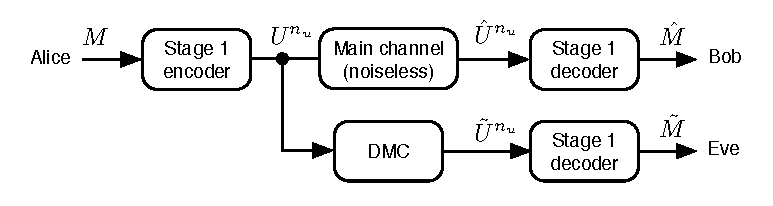
\includegraphics[width=\columnwidth]{WTC.pdf}
%\caption{Here is where the caption goes.}
%\label{fig:wiretap}
%\end{figure}

\section{Problem Set-Up}
\label{sec:prob}
Ideally, the problem of transmitting is to ensure reliability to any intended receiver, and security against any eavesdropper.  
That is, if $B_{p}$ is the probability that Bob receiving the transmitted message, and $E_{p}$ is the probability that Eve receives that message, then at the end of the transmission, then $B_{p} = 1$ and $E_{p} = 0$.  
The piece of this problem that we address is to calculate the average secrecy capacity, defined as the average across all transmissions of the main channel capacity minus the wiretap channel capacity, and the average secrecy probability, which is defined as the average probability that Bob received a packet and Eve dropped that same packet for any given transmission as a function of the angle $\theta$ for a given random variable $\Phi$ and associated input $\phi$, as depicted in Fig \ref{fig:Sig}.  
We do this by calculating the \ac{PEP}, denoted with the variable $\Psi$.  
This is because the equipment we assume to be in use, which is packet based, will receive a packet and either accept it as accurate, or reject it in it's entirety.  
Thus, for a single transmission from Alice with packets of length $M$, then the secrecy capacity is 
\begin{align*}
C_s &= \left(\left(1-\Psi\left(\Phi\left(\phi\right),0\right)\right) - \left(1 - \Psi\left(\Phi\left(\phi\right),\theta\right)\right)\right)M\\
&=  \left(\Psi\left(\Phi\left(\phi\right),\theta\right) -  \Psi\left(\Phi\left(\phi\right),0\right)\right)M
\end{align*}
and, since the probability that Bob receives the packet is independent of the probability that Eve receives the packet, the secrecy probability is
\begin{align*}
P_s &= \left(1-\Psi\left(\Phi\left(\phi\right),0\right)\right)\Psi\left(\Phi\left(\phi\right),\theta\right)
\end{align*}
While the overall goal would be to maximize these two values, we numerically calculate these values for different choices of $\Phi$ and $\phi$ as functions of $\theta$.  
To allow this to drive our model, we shall assume that to encode the message, Alice will use a scheme like the one outlined by Adi Shamir in REFERENCE HOW TO SHARE A SECRET, that allows us to break a message into $n$ encoded packets of length $M$ in such a way that any $k$ packets will ensure full message recovery while $k-1$ or fewer packages guarantee that the message cannot be fully recovered.  
We do not outline the specifics here, but the process develops what is called a \textit{$(k,n)$ threshold scheme}, which we will assume is being used for all transmissions.  
After dividing the message into these packets, we select $k$ packets to transmit, so that reconstruction of the message fails if any antenna fails to receive a single packet.  
Thus reliability is achieved if Bob receives $k$ distinct packets, and security is achieved if Eve receives no more than $k-1$ distinct packets, as desired.  
In order to transmit these packets, we will use the process of beamforming.  
\begin{figure}
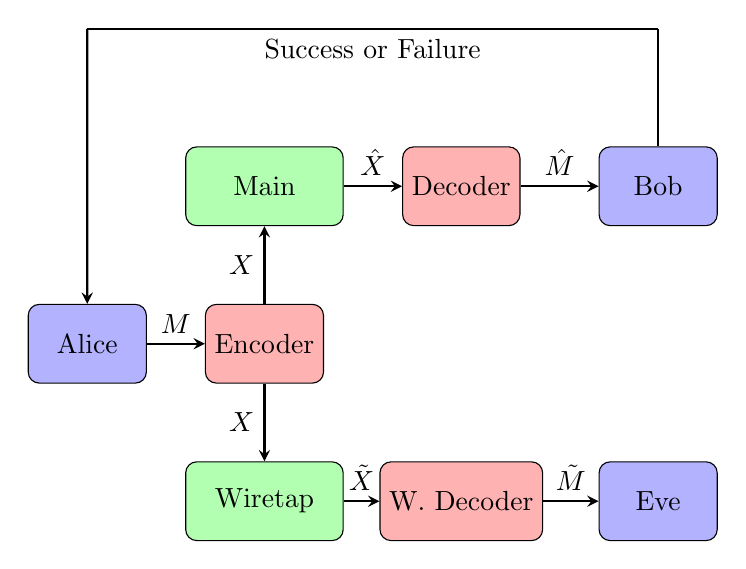
\begin{tikzpicture}[node distance=2cm]
\centering

\node(alice)[communicator]{Alice};
\node(enc)[proc, right of=alice,xshift=0.25cm]{Encoder};
\node(mchan)[chan, above of=enc]{Main};
\node(dec)[proc, right of=mchan, xshift=0.5cm]{Decoder};
\node(bob)[communicator, right of=dec, xshift=0.5cm]{Bob};
\node(echan)[chan, below of=enc]{Wiretap};
\node(edec)[proc, right of=echan,xshift=0.5cm]{W. Decoder};
\node(eve)[communicator, right of=edec,xshift=0.5cm]{Eve};

\coordinate [above of=bob] (u1);
\coordinate[left of=u1,xshift=-5.25cm] (u2);

\draw [arrow] (alice) -- node [anchor=south] {$M$} (enc);
\draw [arrow] (enc) -- node [anchor=east] {$X$} (mchan);
\draw [arrow] (enc) -- node [anchor=east] {$X$} (echan);
\draw [arrow] (mchan) -- node [anchor=south] {$\hat{X}$} (dec);
\draw [arrow] (dec) -- node [anchor=south] {$\hat{M}$} (bob);
\draw [arrow] (echan) -- node [anchor=south] {$\tilde{X}$} (edec);
\draw [arrow] (edec) -- node [anchor=south] {$\tilde{M}$} (eve);
\draw [connect] (bob) -- (u1);
\draw [connect] (u1) -- node [anchor=north] {Success or Failure}(u2);
\draw [arrow] (u2) -- (alice);
\end{tikzpicture}

\caption{Wiretap Channel Model With Feedback}
\label{fig:WCMF}
\end{figure}

\subsection{Beamforming}
\label{sub_sec:beam}

%As stated before, we assume a variant of the wiretap channel model.  
%This variant is depicted in Fig. \ref{fig:WCMF}, and allows Bob to send feedback to Alice.  
%However, we limit Bob to sending messages to simply confirm that a packet was received, or inform that it was rejected.    
%\subsection{Beamforming}
%\label{sub_sec:beam}
%\begin{figure}
%\centering
%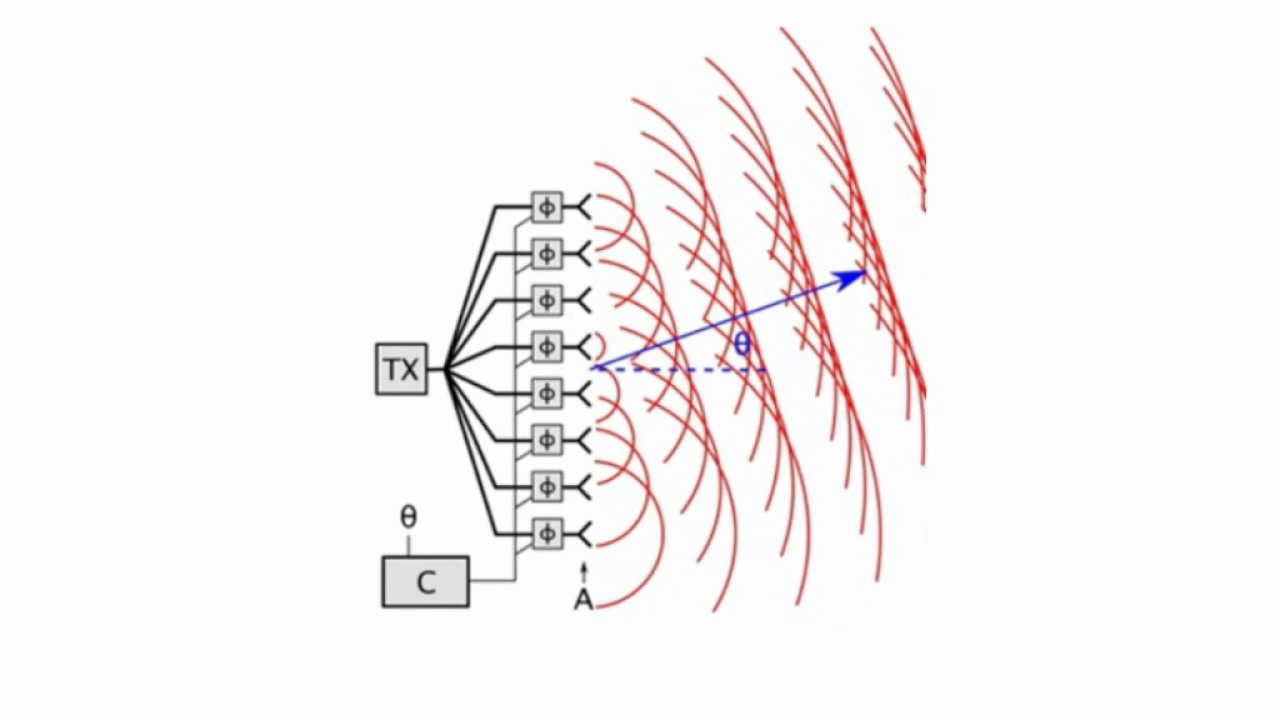
\includegraphics[width=0.9\columnwidth]{Signal.jpg}
%\caption{Transmit Beamforming Set-Up}
%\label{fig:Sig1}
%\end{figure}
Beamforming is a means of using multiple antenna to increase signal power in a certain direction relative to either the transmitter or receiver.  
If done at the transmitter, as is in our model, this is achieved by phase shifting the signal from each antenna to generate constructive interference at the desired angle (in this case, $\theta=0$), as shown in Fig. \ref{fig:Sig}.  
For the entirety of this paper, we will assume that the receiver, Bob, and the eavesdropper, Eve, are in the far field from Alice; that is, they are far enough away that the signal from each of Alice's transmitters appear as a plane, instead of curved.  
Since each antenna is transmitting the same signal, the phase shift needed will correspond to a time delay in the transmission of each antenna.  
This can be represented by 
\begin{equation}
y(t) = \sin\left(2\pi f (t+\delta t)\right) = \sin\left(2 \pi f t + \alpha\right)
\end{equation}
where $f = \frac{c}{\lambda}$ is the transmit frequency, $c$ the speed of light, $\lambda$ is the wavelength, $t$ is time, and $\delta t$ is the time delay needed to achieve the phase shift $\alpha = 2\pi f \delta t$.  
If $\theta$ is the angle toward a receiver off the positive x-axis, then we have
\begin{align*}
\sin(\theta) &= \frac{c \delta t}{\frac{\lambda}{2}} \\
&= \frac{\frac{c\alpha}{2\pi f}}{\frac{\lambda}{2}} \\
&= \frac{c \alpha}{\pi f \lambda} \\
&= \frac{c\alpha}{\pi c} \\
&= \frac{\alpha}{\pi} \\
\Rightarrow \alpha &= \pi \sin(\theta)
\end{align*}
Thus, if we want to steer the beam in the direction $\theta$, we need a phase shift of $\pi \sin(\theta)$ from one antenna to the next.  
So we weight the output of each antenna by $e^{\alpha k i} = e^{\pi \sin(\theta) k i}$ where $k$ is the index of the antenna (in this case, from bottom to top, starting with $0$, with the origin of our system is located at the middle of the antenna array).  
For all transmissions, we will assume that Alice and Bob have already established a connection as outlined in REFERENCE DATBLRF so that Alice knows the optimal phase shift to Bob, which we will place in the direction perpendicular to Alice's antenna array, or rather, in the direction of $\theta = 0$ on a polar graph.  
Alice then calculates the half power beam width, which is the two angles on either side of the optimal angle that receive half the power of the main angle.  
This gives her an angle range $[\theta_{min},\theta_{max}]$ where, since Bob is oriented towards $\theta = 0$, we should have $\theta_{min} \approx -\theta_{max}$, so we choose $\phi = 2\theta_{max}$.
An image providing the \ac{SINR} as for a beam directed at $\theta = 0$ can bee seen in Fig. \ref{fig:polar}.

\begin{figure}
\centering
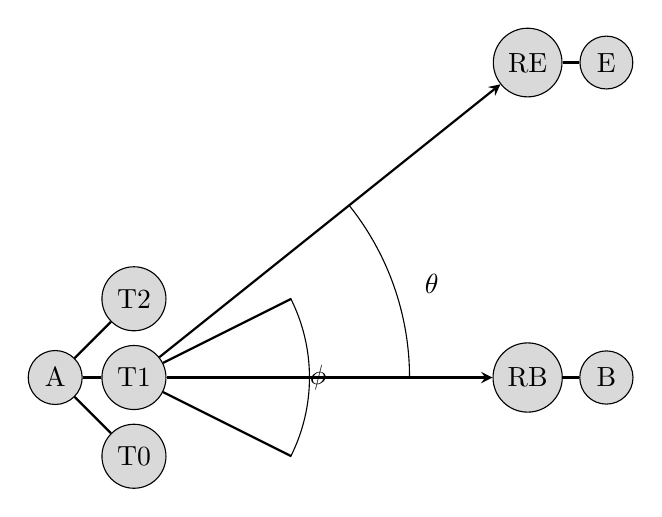
\begin{tikzpicture}

\node(a1)[antenna]{A};
\node(k1)[antenna, right of=a1]{T1};
\node(k0)[antenna, below of=k1]{T0};
\node(k2)[antenna, above of=k1]{T2};
\node(b1)[antenna, right of=k1,xshift=5cm]{B};
\node(r0)[antenna, left of=b1]{RB};
\node(e1)[antenna, above of=b1,yshift=3cm]{E};
\node(r1)[antenna, left of=e1]{RE};

\coordinate [right of=k2,xshift=1cm] (pt);
\coordinate [right of=k0,xshift=1cm] (pb);

\draw [connect] (a1) -- (k0);
\draw [connect] (a1) -- (k1);
\draw [connect] (a1) -- (k2);
\draw [connect] (r1) -- (e1);
\draw [connect] (r0) -- (b1);
\draw [arrow] (k1) -- node (hid1) [anchor=north] {} (r0);
\draw [arrow] (k1) -- node (hid2) [anchor=south] {} (r1);
%\draw [connect] (hid1) to[out=45,in=-30] node [anchor=west] {$\theta$} (hid2);
\draw pic[draw,angle radius=3.5cm,"$\theta$" shift={(18mm,5mm)}] {angle=r0--k1--r1};
\draw [connect] (k1) -- (pt);
\draw [connect] (k1) -- (pb);
\draw pic[draw,angle radius=2.22925cm,"$\phi$" shift={(10mm,0mm)}] {angle=pb--k1--pt};

\end{tikzpicture}
\caption{An example of the transmission set-up where Alice utilizes three transmitters, and Bob and Eve both have one receiver.}
\label{fig:Sig}
\end{figure}

\begin{figure}
\centering
\includegraphics[width=0.9\columnwidth]{"SINR Colormap".png}
\caption{SINR by Location}
\label{fig:polar}
\end{figure}
%Coset codes for secrecy can be represented by code tables like the one in Table~\ref{tab:code}.

%\begin{table}[]
%\centering
%\caption{Codebook structure for a coset-based secrecy code.}
%\label{tab:code}
%\begin{tabular}{c|cccc}

%$M$ & \multicolumn{4}{c}{Codewords}           \\ \hline \hline
%0 & 0000 & 0011 & 1100 & 1111 \\ 
%1 & 0001 & 0010 & 1101 & 1110 \\
%2 & 1000 & 1011 & 0100 & 0111 \\ 
%3 & 1001 & 1010 & 0101 & 0110 \\ 
%\end{tabular}
%\end{table}

%\subsection{Generating a Discrete Memoryless Channel}
%\label{sec:generatingDMC}


%\begin{figure}
%\centering
%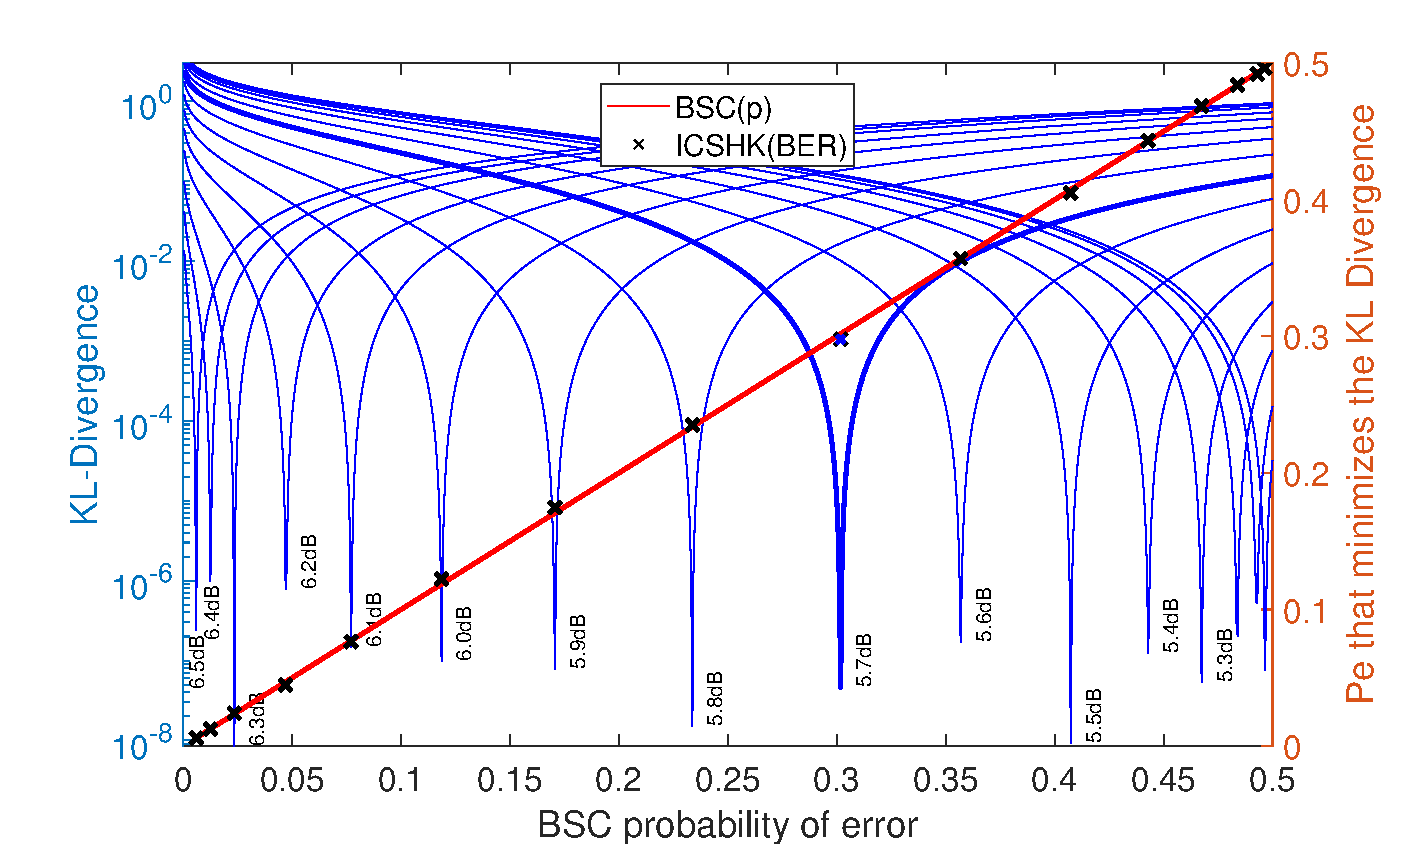
\includegraphics[width=0.9\columnwidth]{kld2.pdf}
%\caption{Kullback-Leibler divergence for SNR between 5dB and 6.5dB}
%\label{fig:kld}
%\end{figure}

%Fig. \ref{fig:kld} shows 16 curves representing the different SNR values of the ICSHK channel from 5dB to 6.5dB. By representing the curves in logarithmic scale we can detect which is the minimum value and so we can observe to which SNR value what probability of error it corresponds and associate it with a BER.

%Probably will need sections with titles like the following sections

\section{Impact of Randomized Beamforming on \ac{PEP}}

The main benefit of the beamforming is to take advantage of possible differences in the physical locations of Bob and Eve.  
If Eve is at a different enough angle from Alice than Bob that she is not in the main beam for the transmission of a specific packet, then the \ac{SINR} at Bob will be much better than the \ac{SINR} at Eve, making it more likely that Eve won't receive the packet but Bob will.  
While this is great if Eve truly is positions as in Fig. \ref{fig:polar}, it doesn't help very much if Eve is close enough to co-linear with Alice and Bob that she remains in the main beam of transmission as well as Bob.  
This is part of the reason for exploring the effect of randomization in the direction of the beam, as well as impairing the \ac{SINR} inside the main beam of transmission.  
Since a beam pointed directly at Bob will result in the highest \ac{SINR} being in the direction from Alice to Bob, if Alice just points the beam directly at Bob, then she is also pointing the beam directly at Eve.  
So, in this worst case scenario, how do we impair the transmission so that we can still achieve secrecy?  

To answer that question, we should calculate what the optimal \ac{PEP} should be from a secrecy probability standpoint.  
To do so, we consider the following optimization problem:
\[ \begin{matrix} \textnormal{max}_{B_P,E_P} & B_P(1-E_P) \\ \textnormal{s.t.} & E_P = B_P \\ & 0 \leq E_P,B_P \leq 1 \end{matrix} \]
where $B_P,E_P$ is the probability that Bob and Eve receive a given packet respectively, as previously defined.  
The condition that $E_P = B_P$ comes from the fact that with this transmission scheme, we're guaranteed that for some packets in the transmission sequence (the exact number will be dependent on the random variable $\Phi$) we will have $E_{P} \leq B_{P}$.  
These are the packets we have the best chances of communicating secretly, so we focus on them.  
In this case, however, the worst case scenario is that $E_{p} = B_{p}$.  
Using Lagrange multipliers, it is easy to see that the solution to this problem is $B_P = E_P = \frac{1}{2}$, so the most probable way to get Bob to receive a packet that gets erased on Eve's channel is if the minimum \ac{PEP} inside the main beam is $50\%$.  
This is the minimum \ac{PEP} because it is better for both Eve and Bob to drop the packet, than it is for both Eve and Bob to receive the packet.  
Every time Bob drops the packet, he will simply request a retransmission, which will give Eve another shot at receiving the packet, essentially making it equivalent (security wise) to a situation where we just haven't transmitted that packet yet.  
If they both receive it, however, than we've already leaked information to Eve.  
Since the goal for these first few patterns is to achieve security, in a choice between Eve receiving a packet or Bob dropping a packet, we prefer to have Bob drop the packet.

In a SISO channel where Alice has multiple antennas and there is Rayleigh fading, the received signal is
\begin{equation}
y = \sqrt{P}\textbf{h}^{H}\textbf{w}s + n
\end{equation}
where $\textbf{h} = \left[ \begin{matrix} h_{0} & ... & h_{N-1} \end{matrix} \right]^{T}$ with $h_{k} \in \mathscr{CN}(0,\sigma_{h}^{2})$, $n \in \mathscr{N}(0,\sigma_{n}^{2})$, and $P$ is the power of the signal in Bob's direction.  
Thus, the \ac{SINR} is defined as
\begin{equation}
\Gamma = \frac{P}{\sigma^{2}}\left|\textbf{h}^{H}\textbf{w}\right|^{2}
\end{equation}
For simplicity, we will assume that both the Rayleigh fading and the \ac{AWGN} have mean $0$ and unit variance, that is $\sigma_{h} = \sigma = 1$.  
From this \ac{SINR} and the the assumption that we will transmit with \ac{QPSK}, we then can directly calculate the \ac{BER} as $Q(\sqrt{2\Gamma})$ where
\begin{equation}
Q(x) = \frac{1}{\sqrt{2\pi}}\int_{x}^{\infty} e^{-\frac{u^{2}}{2}} \,\mathrm{d}u
\end{equation}
Finally, if it is possible to correct $t$ bit errors in a packet of $M$ bits, then the \ac{PEP} is the probability that we have at least $t+1$ errors, or rather
\begin{equation}
\Psi = \sum_{i=t+1}^{M} \binom{M}{i} \epsilon_{c}^{i}(1-\epsilon_{c})^{M-i}
\end{equation}
We will consider the packet as corrupted (and thus discard it) if any bit is received in error, thus
\begin{align*}
\Psi &= \sum_{i=1}^{M} \binom{M}{i} \epsilon_{c}^{i}(1-\epsilon_{c})^{M-i} \\
&= 1 - \binom{M}{0} \epsilon_{c}^{0}(1-\epsilon_{c})^{M} \\
&= 1 - \left(1-Q\left(\sqrt{2\Gamma_{c}}\right)\right)^{M} \\
&= 1 - \left(\frac{1}{\sqrt{2\pi}}\int_{-\infty}^{\sqrt{2\Gamma_{c}}} e^{-\frac{u^{2}}{2}} \,\mathrm{d}u\right)^{M}
\end{align*}
While this is obviously ideal, the \ac{SINR} will vary from transmission to transmission, and as such, there is no way to guarantee that \ac{PEP} is always 50\%.  
However, through careful transmission selection, a code can be designed to put the average \ac{PEP} for the best location (which is Bob's position) near 50\%.  

With this, we now have to consider which distributions we should use as random variables in order to determine which directions we point the beams.  
As stated before, the obvious choice is to not include a random variable, and just point all the beams directly at Bob to transmit the packets.  
However, the question we want to answer is whether or not choosing a random variable to distribute the beam directions will help increase secrecy, without damaging the reliability.  
In this paper, we consider three different distributions: a uniform distribution, a truncated normal distribution, and a sinusoidal distribution.  
Since these are a function of $\phi$, for the uniform distribution, we have
\begin{equation}
\Phi_U\left(x,\phi\right) = \begin{cases} \frac{1}{\phi} & -\frac{\phi}{2} \leq x \leq \frac{\phi}{2} \\ 0 & \textnormal{otherwise} \end{cases}
\end{equation}
the truncated normal distribution is defined as
\begin{equation}
\Phi_{TN}\left(x,\phi\right) = \begin{cases} \frac{e^{-x^{2}/2}}{\sqrt{2\pi}\left(1 - 2Q\left(\frac{\phi}{2}\right)\right)} & -\frac{\phi}{2} \leq x \leq \frac{\phi}{2} \\ 0 & \textnormal{otherwise} \end{cases}
\end{equation}
and the sinusoidal distribution as
\begin{equation}
\Phi_{S}\left(x,\phi\right) = \begin{cases} \frac{1-\cos\left(\frac{2\pi}{\phi}x\right)}{\phi\left(1-\frac{1}{\pi}\sin\left(\frac{2\pi}{\phi}\right)\right)} & -\frac{\phi}{2} \leq x \leq \frac{\phi}{2} \\ 0 & \textnormal{otherwise} \end{cases}
\end{equation}
While many values of $\phi$ were chosen, the most interesting are $\phi = 0$, and when $\phi$ is the half-beam width of the beam directly pointed at Bob, which in this case, was $\phi = \frac{\pi}{18}$.
%Since we want $\ac{PEP} \geq 0.5$, we then have
%\begin{align*}
%\ac{PEP} &\leq 1 - \left(\frac{1}{\sqrt{2\pi}}\int_{-\infty}^{\sqrt{2\Gamma}} e^{-\frac{u^{2}}{2}} \,\mathrm{d}u\right)^{M} \\
%\Rightarrow 1-\ac{PEP} &\geq \left(\frac{1}{\sqrt{2\pi}}\int_{-\infty}^{\sqrt{2\Gamma}} e^{-\frac{u^{2}}{2}} \,\mathrm{d}u\right)^{M} \\
%\Rightarrow \left(1-\ac{PEP}\right)^{\frac{1}{M}} &\geq \frac{1}{\sqrt{2\pi}}\int_{-\infty}^{\sqrt{2\Gamma}} e^{-\frac{u^{2}}{2}} \,\mathrm{d}u \\
%\Rightarrow \left(1-\ac{PEP}\right)^{\frac{1}{M}} &\geq 1 - Q\left(\sqrt{2\Gamma}\right) \\
%\Rightarrow Q\left(\sqrt{2\Gamma}\right) &\geq 1 - \left(1-\ac{PEP}\right)^{\frac{1}{M}} \\
%\Rightarrow \ac{BER} &\geq 1 - \left(1-\ac{PEP}\right)^{\frac{1}{M}}
%\end{align*}
%Thus, if every bit is needed for proper decoding, then we simply need $\ac{BER} \geq 1 - (1-\ac{PEP})^{\frac{1}{M}}$ where $M$ is the packet length for a desired \ac{PEP}.

\section{Results and Analysis}
To achieve these results, numbers were calculated as if using $7$ transmitting antennas oriented vertically, with a single receiving antenna.  
These numbers were calculated for $500$ different points evenly spaced on a circle of unitary distance from the transmitter.  
Each of the $100$ packets was set to be $10$ bits long, and transmitted at the same power level, without any encoding (though those numbers were included in coding so that they can be adjusted).  
The probabilities were calculated using $1000$ simulations of transmitting these packets.  
\begin{figure}
\centering
\includegraphics[width=0.9\columnwidth]{"Secrecy_Probability_0".png}
\caption{Secrecy Probability: The overall probability that Bob receives a packet Eve drops that packet $\phi=0$ (so all distributions are the same).}
\label{fig:secprob0}
\end{figure}

\begin{figure}
\centering
\includegraphics[width=0.9\columnwidth]{"Secrecy_Probability".png}
\caption{Secrecy Probability: The overall probability that Bob receives a packet Eve drops that packet $\phi=\pi/18$.  In order, Uniform, Truncated Normal, and Sinusoidal}
\label{fig:secprobpi18}
\end{figure}

\begin{figure}
\centering
\includegraphics[width=0.9\columnwidth]{"Secrecy_Capacity_0".png}
\caption{Secrecy Capacity: The approximate number of bits we can secretly transmit to Bob per channel use (which sends 10 bits) and a range of $\phi=0$ (so all distributions are the same).}
\label{fig:seccap0}
\end{figure}

\begin{figure}
\centering
\includegraphics[width=0.9\columnwidth]{"Secrecy_Capacity".png}
\caption{Secrecy Capacity: The approximate number of bits we can secretly transmit to Bob per channel use (which sends 10 bits) and a range of $\phi=\pi/18$.  In order, Uniform, Truncated Normal, and Sinusoidal}
\label{fig:seccappi18}
\end{figure}

In Fig \ref{fig:secprob0} and Fig \ref{fig:secprobpi18}, we have a graph of the secrecy probability as a function of $\theta$.    
Fig \ref{fig:secprob0} is this probability when transmission beams are directed at Bob, and only Bob, while Fig \ref{fig:secprobpi18} is the probabilities when transmission beams are randomly selected from within the half-beam width of the beam pointing directly at Bob.  
In the progression from $\phi = 0$ to $\phi = \frac{\pi}{18}$, the probability decreases on average by $1\%$, from approximately $33\%$ to approximately $32\%$ at best and $23\%$ to $22\%$ at worst.  
This decrease happens at a more or less steady pace, and continues to decrease as $\phi$ extends further outside the half-beam width.  
This is reflected rather accurately in the figures representing the secrecy capacity graphs in Fig \ref{fig:seccap0} and Fig \ref{fig:seccappi18} (both of which are a measurement of secrecy capacity as a function of $\theta$).  
As we can see, utilizing beamforming to increase security at the physical layer is feasible, and can allow for security to be improved strictly by the angle from Bob to Eve,  
Unfortunately, none of the random distributions actually improved the security.  
However, what this scheme doesn't account for, and can be continued in later work, is the possibility of using the random distributions to determine pointing the antenna in different directions while maintaining the central beam pointed directly at Bob.  
This process could provide the added secrecy that this simple scheme did not.

\section{Conclusion}
\label{sec:conc}
While this scheme is obviously very rough and not very advanced, it does indicate that transmission security can be improved by utilizing beamforming, without decreasing reliability.  
Just by utilizing beamforming, we can have the probability for Bob receiving a packet that Eve drops around 30\%, and get an average secrecy capacity of $2.78$ bits per $10$ bit channel use.  
Randomizing the beamforming direction does not seem to increase the secrecy of the transmission at this simpler level, but further explorations will be needed to fully rule this out as a useful schematic. 

Coupled with the security themes in~\cite{Harrison2010}, this scheme can improve security for the physical layer against attackers using publicly available off the shelf equipment.




% \addtolength{\textheight}{-12cm}   % This command serves to balance the column lengths
                                  % on the last page of the document manually. It shortens
                                  % the textheight of the last page by a suitable amount.
                                  % This command does not take effect until the next page
                                  % so it should come on the page before the last. Make
                                  % sure that you do not shorten the textheight too much.


\bibliographystyle{IEEEtran}
\bibliography{IEEEabrv,biblio}


\end{document}
